
Para clarificar algunas de las partes del código que consideramos más difíciles de plasmar en un diagrama estático, incluimos diagramas de secuencia para diversas partes del trabajo práctico. Estas partes corresponden a diversas situaciones donde mostramos como podría ser una implementación de la lógica secuencial que se desarrolla.

\subsubsection{Inicio de un seguimiento}\label{diag_inicioSeguimiento}
\begin{center}
	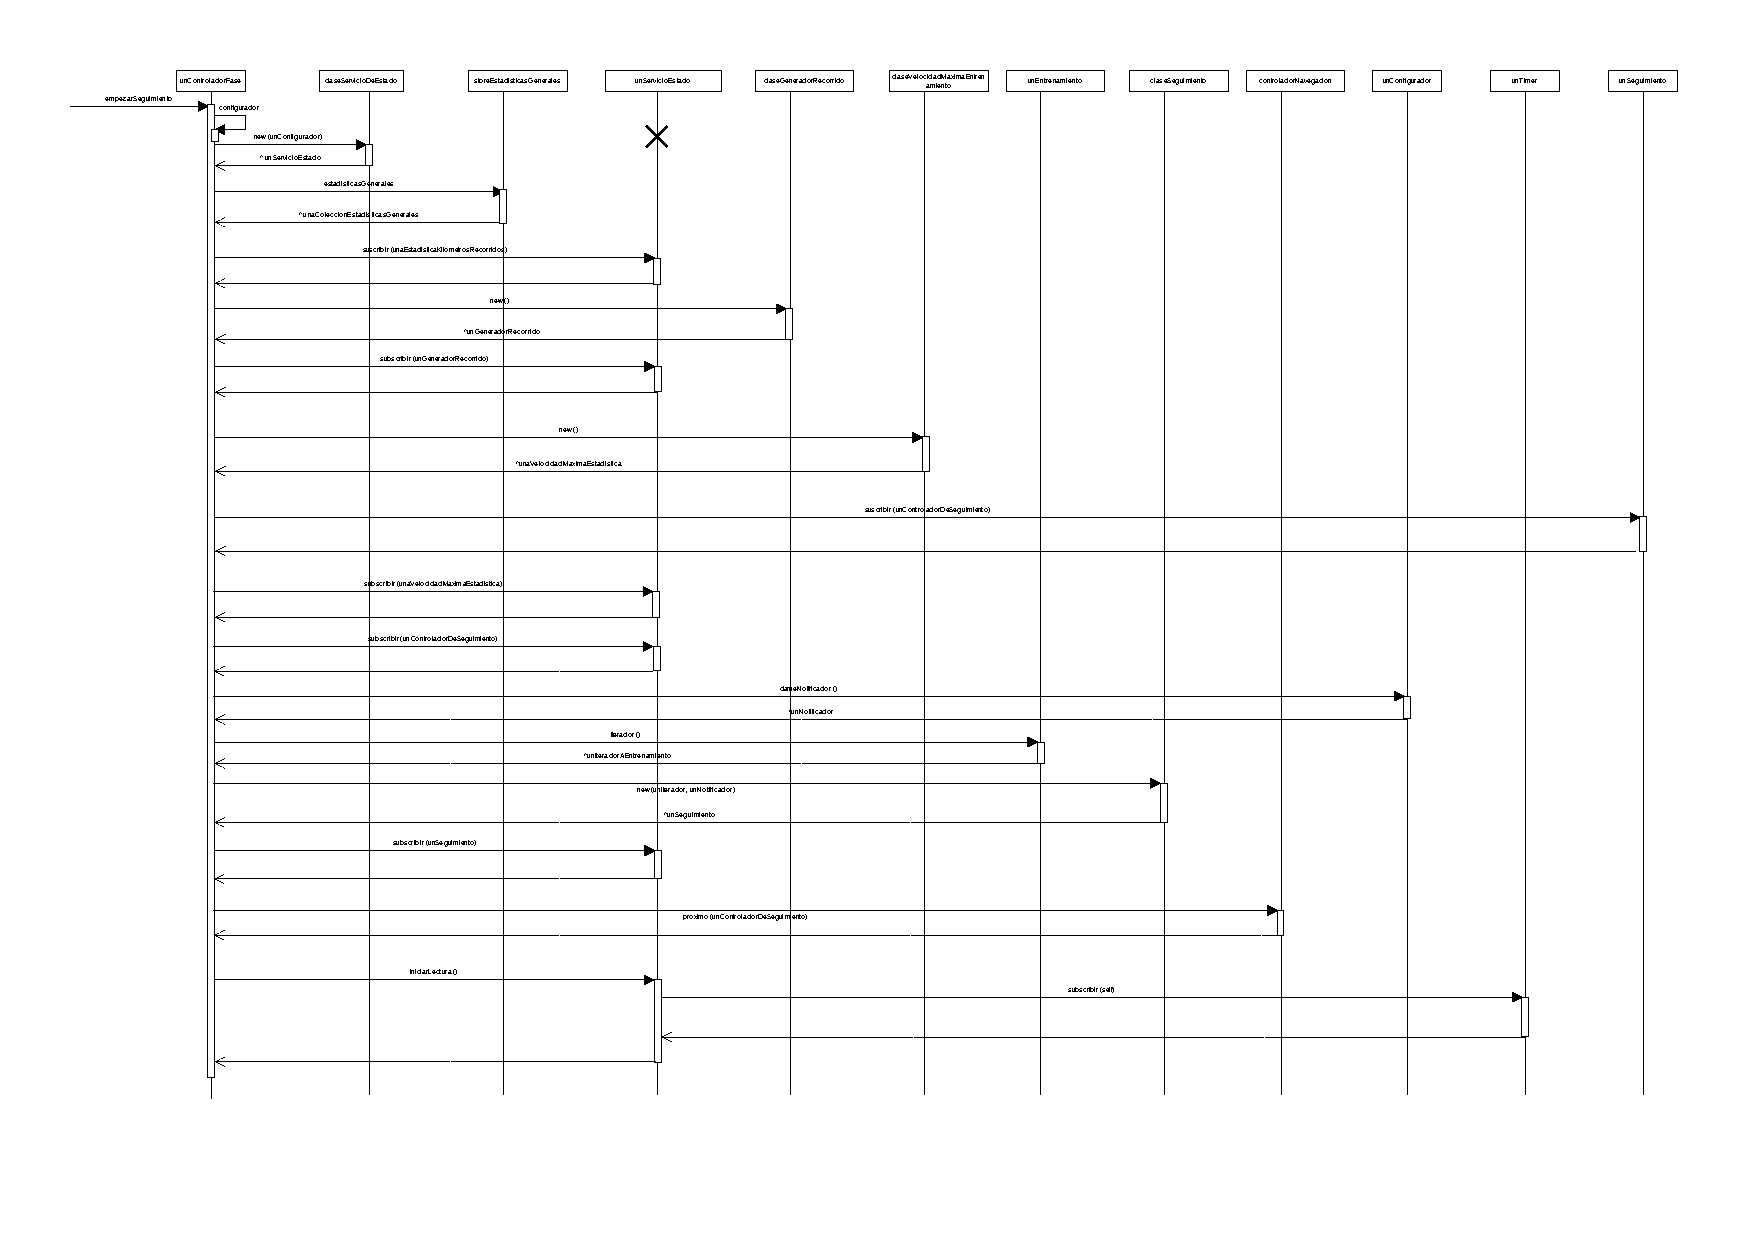
\includegraphics[scale=0.5]{images/InicioSeguimiento.pdf}
\end{center}

Este diagrama de secuencia muestra el proceso de inicio de seguimiento. A grandes razgos, el controlador de fase crea un servicio de estado (que será le encargado de mandar las actualizaciones de estado a otros componentes). Esta interacción es un poco compleja para ponerla en el mismo diagrama, así que se la separó en el diagrama ``Crear un servicio de estados'', que se puede ver en la sección \ref{diag_crearUnServicioDeEstado}. 


Luego se procede a suscribir a todos los objetos que deben recibir actualizaciones de estado al controlador (creándolos si no existían), para lo que se le manda repetidas veces el mensaje \emph{suscribir (unObjeto)} al \texttt{ServicioDeEstado}. Antes de eso, se suscribe al \texttt{ControladorDeSeguimiento} al \texttt{Seguimiento} para que este pueda informarle al primero cuando se finalizó el seguimiento. Esto es posible porque el \texttt{ServicioDeEstados} implementa la interfaz \texttt{SuscriptorDeFinSeguimiento}.


Finalmente, se inicializa el servicio de estados, enviándole el mensaje \emph{iniciarLectura ()}, lo que provoca que éste (que implementa la interfaz \texttt{SuscriptorDeTimer}), le envíe un mensaje \emph{suscribir (self)} al timer. De esa forma queda suscripto el notificador de estados al timer y éste le enviará notificaciones a intervalos regulares.


Suponiendo que el usuario ya realizó la configuración inicial y tiene algún plan con entrenamientos seteados, el camino por el que debe navegar para llegar a este diagrama de secuencia es:
\begin{itemize}
	\item Seleccionar uno de sus planes de la lista de planes disponibles.
	\item Seleccionar un entrenamiento de la lista de entrenamientos del plan.
	\item En esa pantalla (donde se listan las fases correspondientes al entrenamiento) se presiona ``comenzar''.
\end{itemize}

\subsubsection{Actualización dentro de un seguimiento} \label{unaSeccion}
\begin{center}
	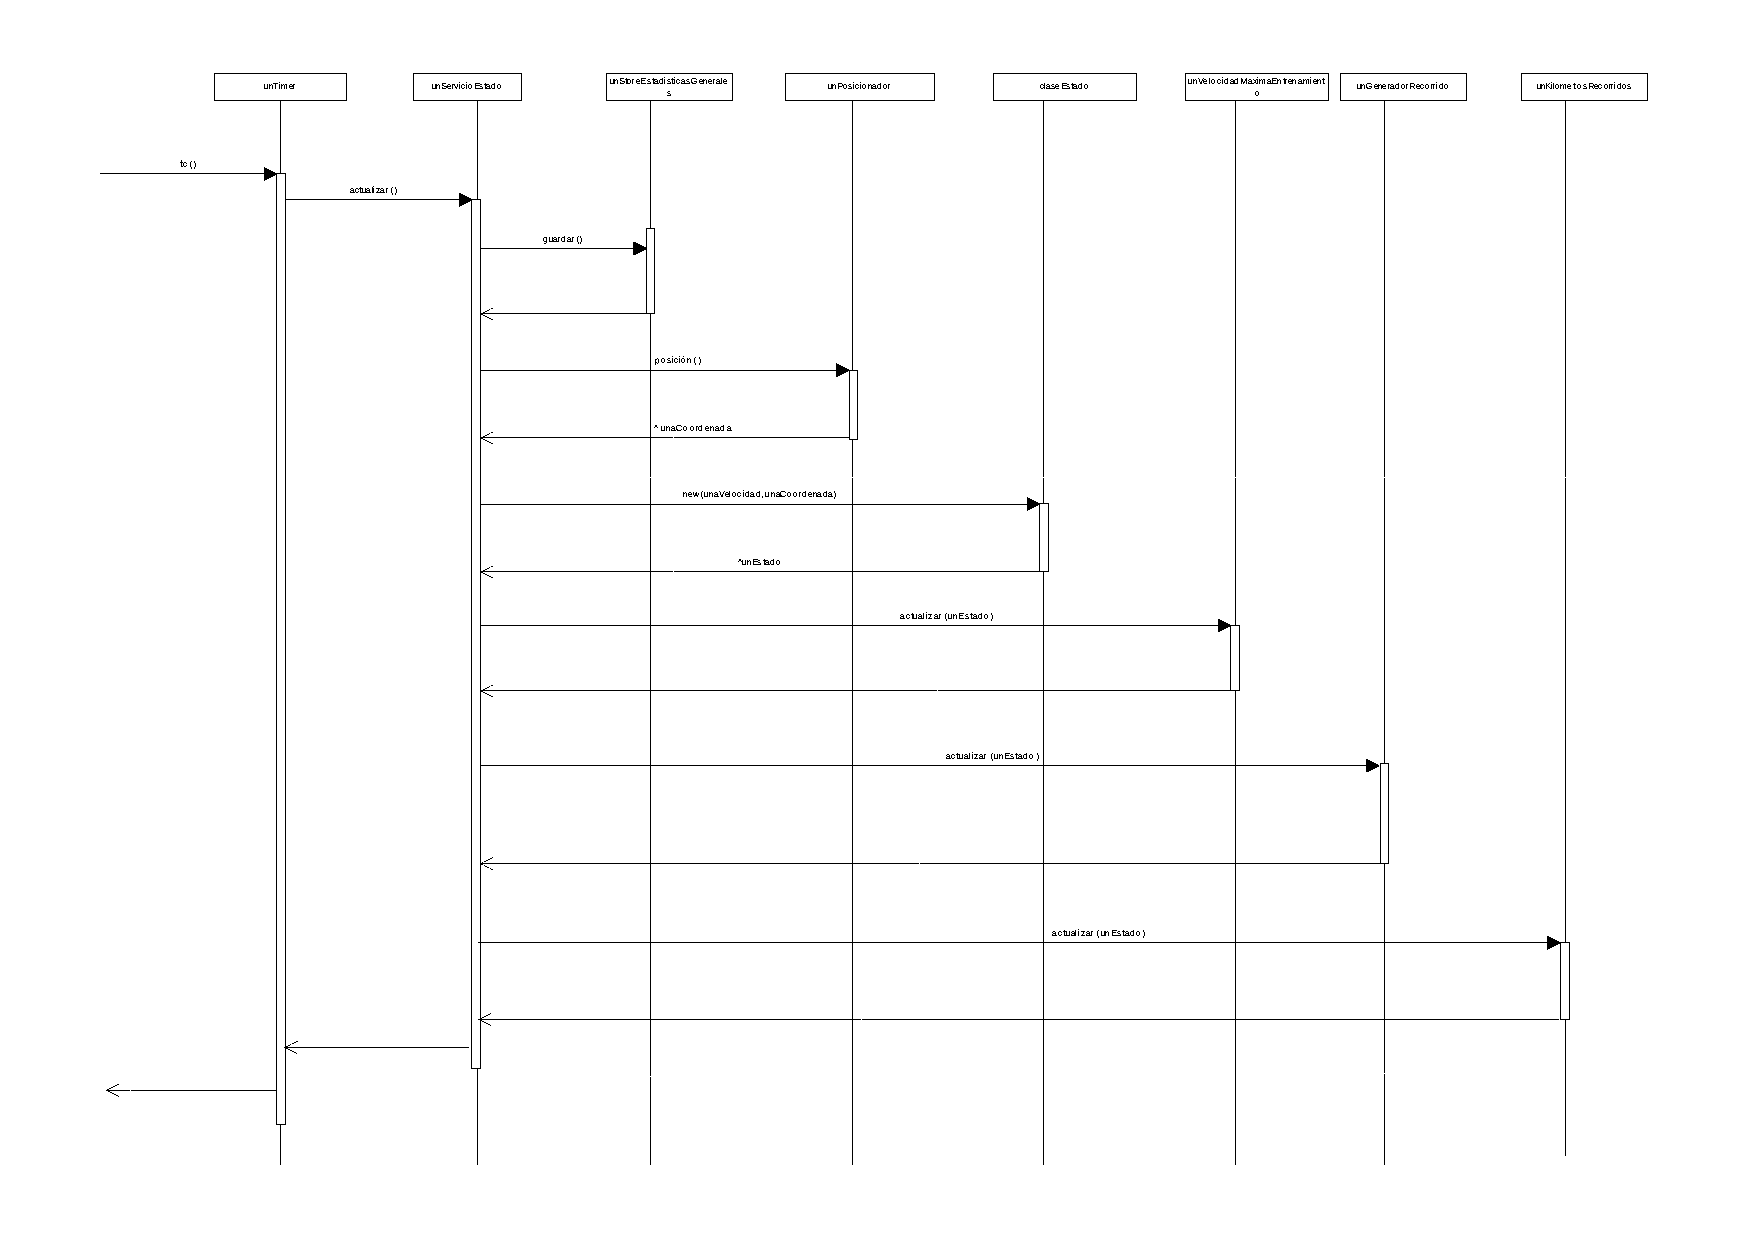
\includegraphics[scale=0.5]{images/actualizacionSeguimiento.pdf}
\end{center}

Este diagrama muestra la secuencia de mensajes intercambiados a la hora de realizar una actualiación dentro de una fase, mientras el usuario está corriendo. Los pasos para llegar a este mensaje son los mismos que el anterior, esperando el tiempo correspondiente a la frecuencia de actualización que se haya realizado.


En primer lugar, el objeto \texttt{Timer} recibe un mensaje \emph{tic ()}. Este mensaje está en el diseño para que éste quede agnóstico a la implementación de la plataforma sobre la que se está trabajando. En el caso particualr de \emph{iOS}, este mensaje no existe sino que se le especifica al sistema operativo que un método en particular (en este caso el \emph{actualizar}) debe ser invocado regularmente cada cierto tiempo. Cuando el \texttt{Timer} recibe ese mensaje, le informa al \texttt{ServicioDeEstado} (pues es el único que está suscripto al \texttt{Timer}) enviándole el mensaje \emph{actualizar ()}.


Al recibir este mensaje, el \texttt{ServicioDeEstado} le solicita a sus colaboradores internos la velocidad y posición actual del teléfono (mediante los mensajes \emph{velocidadActual ()} y \emph{posición ()} respectivamente) y crea un nuevo \texttt{Estado} con esa información.


Finalmente le envía a cada uno de sus suscriptores el mensaje \emph{actualizar (unEstado)}, para que estos puedan realizar sus respectivas acciones con la nueva información del estado. 

\subsubsection{Crear un servicio de estado}\label{diag_crearUnServicioDeEstado}
\begin{center}
	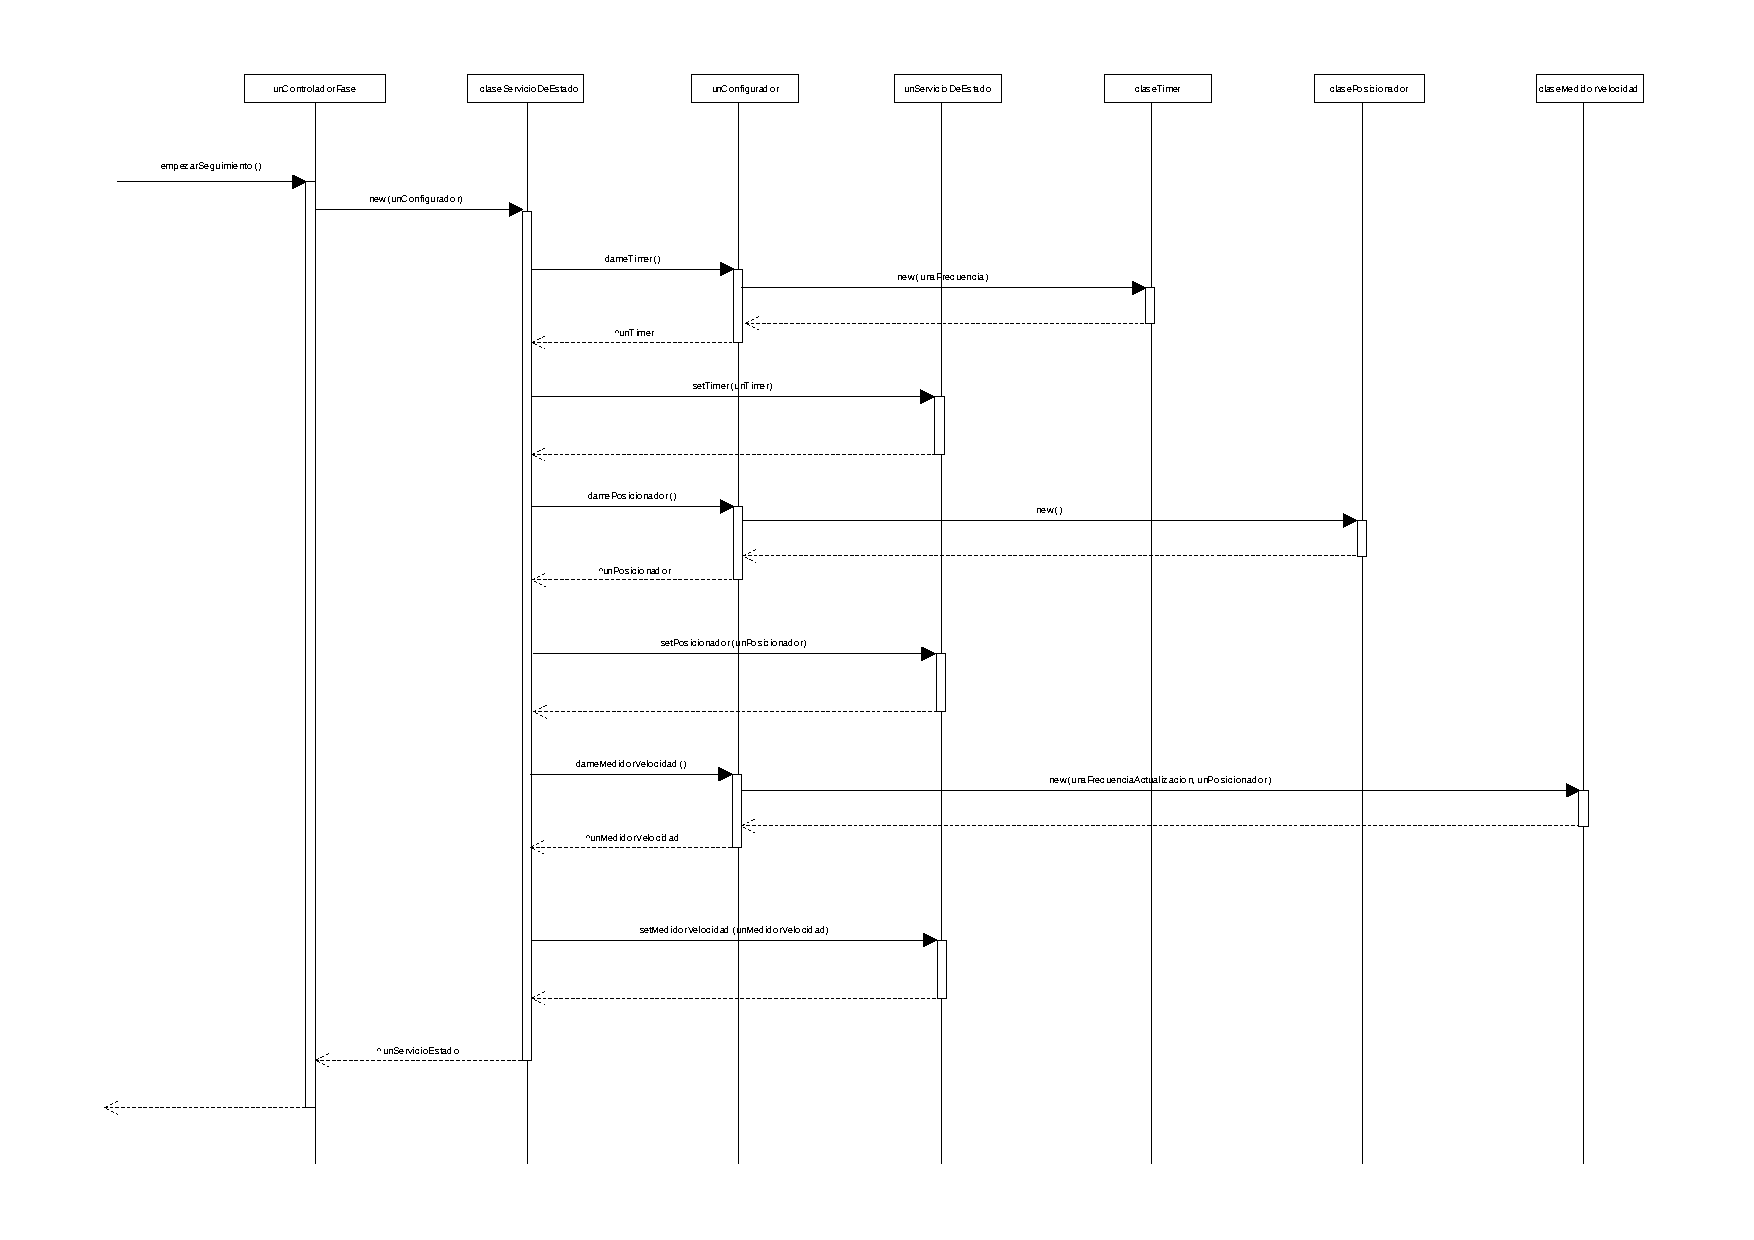
\includegraphics[scale=0.5]{images/CrearServicioEstado.pdf}
\end{center}

En este diagrama se puede observar el proceso de creación de un objeto \texttt{ServicioDeEstado}, que se crea al comenzar el entrenamiento, como se puede ver en la sección \ref{diag_inicioSeguimiento}. Para crear el \texttt{ServicioDeEstado}
 se pasa como parámetro un \texttt{Configurador}, del que se obtienen y setean como colaboradores internos el \texttt{Timer}, el \texttt{Posicionador} y el \texttt{MedidorVelocidad}. El configurador crea dinámicamente estos elementos a medida que se le son solicitados y los devuelve.

 Una vez que todos los elementos están seteados, se devuelve el recién creado \texttt{ServicioDeEstado}, sin que éste se suscriba al \texttt{Timer}.  


Para la creación del servicio de estado se nos planteó una disyuntiva:
\begin{itemize}
	\item Una opción era no guardar el \texttt{Timer} como colaborador interno del \texttt{ServicioDeEstado}, sino que simplemente cuando a la hora de crear el \texttt{ServicioDeEstado}, se pida al \texttt{Configurador} el \texttt{Timer} y el \texttt{ServicioDeEstado} se suscriba en ese momento. Esta alternativa (no elegida) tenía la ventaja de que evitaba almacenar como colaborador interno al \texttt{Timer} y nos ahorraba el método \emph{iniciarLectura ()}. Sin embargo tiene un defecto: si la frecuencia de actualización era demasiado rápida, podía llegar a llamarse al mensaje \emph{actualizar ()} del servicio de estado (por un \emph{tic ()} del sistema operativo) antes de que todos sus colaboradores internos estuvieran registrados, potencialmente perdiendo información de los primeros estados.
	\item La alternativa que se nos ocurrió para esto es que se almacene el \texttt{Timer} como colaborador interno del \texttt{ServicioDeEstado} y que una vez que el controlador termine de suscribir a quienes corresponda, llame a un método del \texttt{ServicioDeEstado}(\emph{iniciarLectura ()}) que se ocupe de suscribirlo al \texttt{Timer}. Elegimos esta alternativa porque pensamos que en un futuro puede existir algún objeto (por ejemplo una nueva \texttt{Estadistica}) para el que sea importante no perder los estados iniciales. 
\end{itemize}


\subsubsection{Finalización de un seguimiento}
\begin{center}
	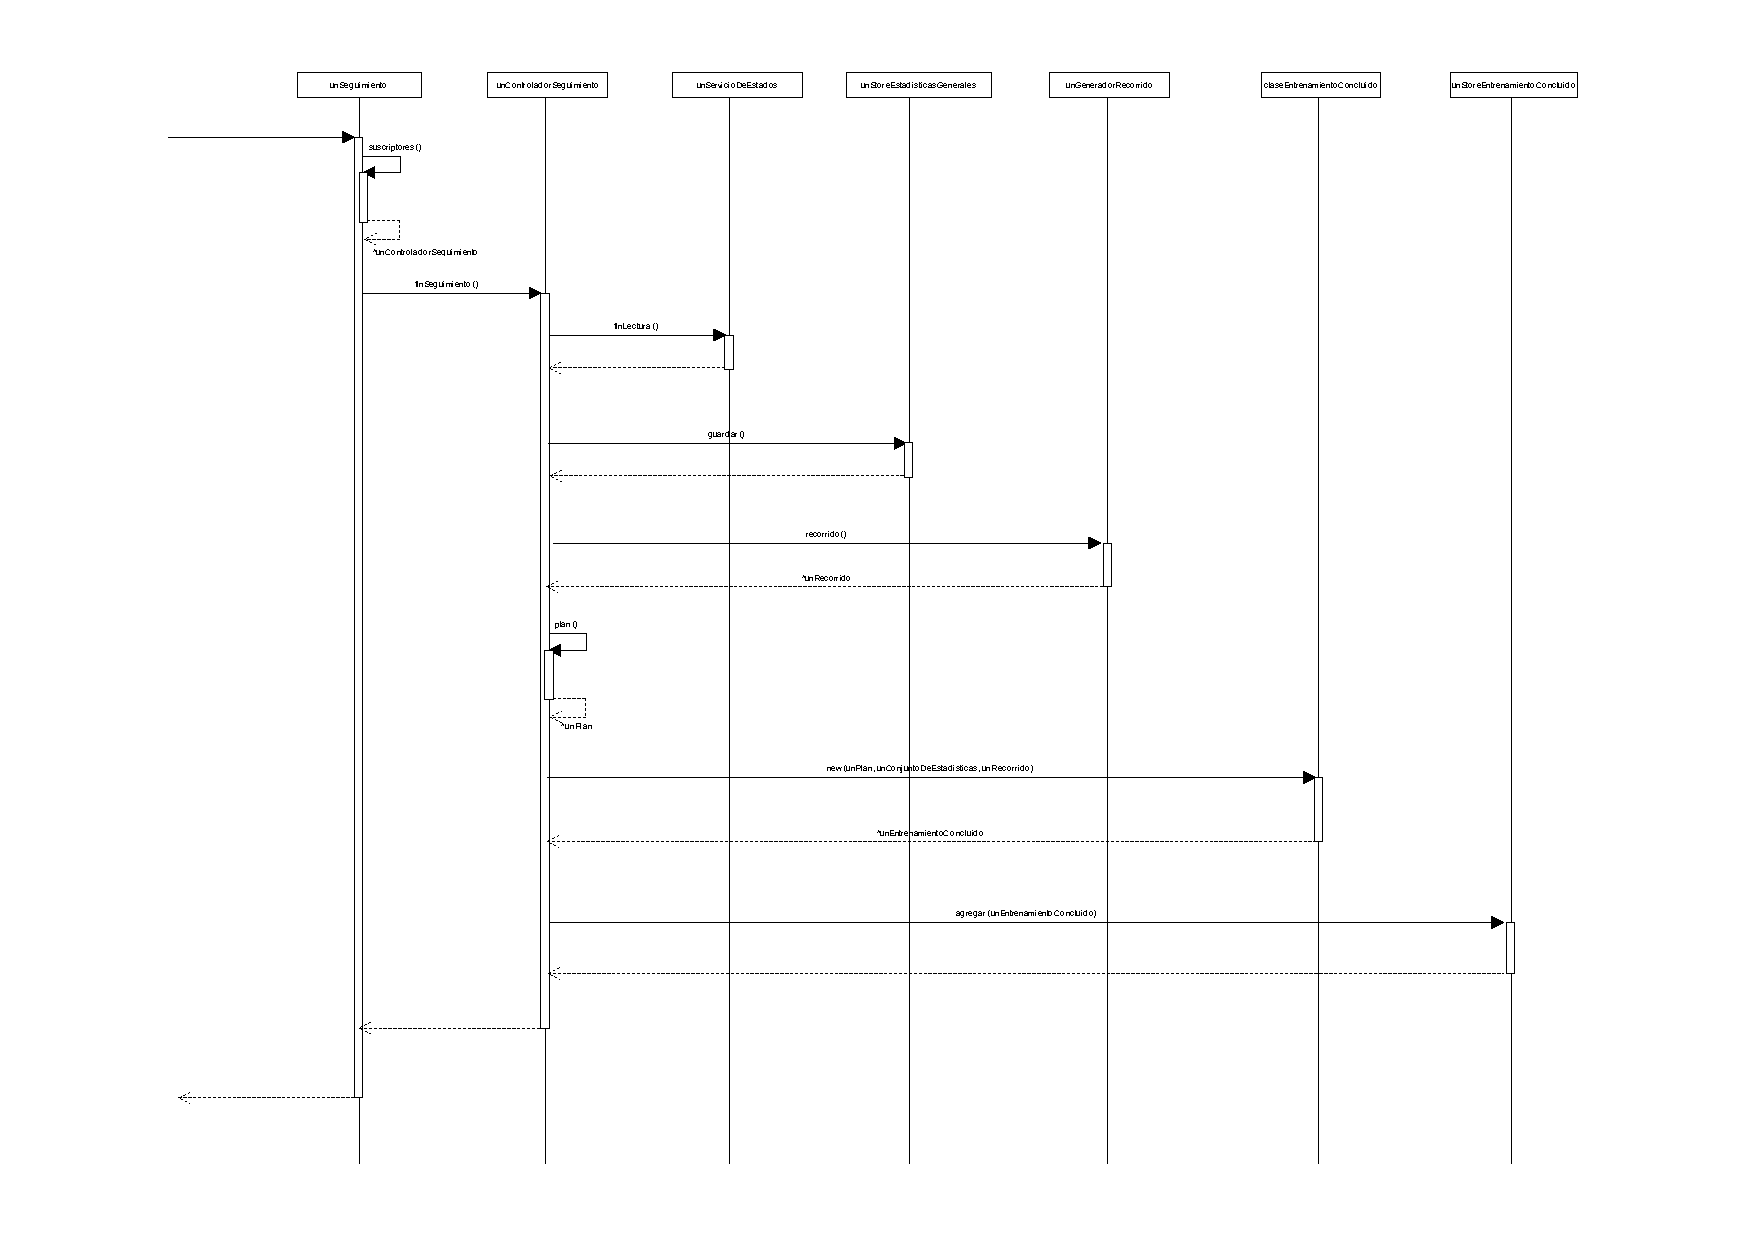
\includegraphics[scale=0.5]{images/FinalizacionSeguimiento.pdf}
\end{center}

Este diagrama muestra cómo es el proceso de finalización de un seguimiento cuando concluye un entrenamiento. El \texttt{Seguimiento}, encargado de seguir el proceso de entrenamiento, se da cuenta de que el entrenamiento finalizó (puede haber sido porque el usuario cumplió el tiempo y distancia correspondientes a la última fase del entrenamiento en curso o porque apretó el botón de ``detener'' en la vista de seguimiento) y se le informa al \texttt{ServicioDeEstados} que deje de tomar lecturas del \texttt{Timer}. Para eso, le envía el mensaje \emph{finLectura ()}. 

Acto seguido, el controlador informa al \texttt{StoreEstadisticasGenerales} que guarde las estadísticas generales que se estuvieron actualizando durante el entrenamiento (mediante el mensaje \emph{guardar ()}) y procede a crear un nuevo objeto \texttt{EntrenamientoConcluido} para almacenarlo en su correspondiente \texttt{StoreEntrenamientoConcluido}. Para eso, obtiene el \texttt{Recorrido} del \texttt{GeneradorDeRecorridos} y, usando sus colaboradores internos \texttt{Plan} y \texttt{CollectionEstadisticasEntrenamiento}, llama al \emph{new (unPlan, unaColeccionDeEstadisticas, unRecorrido)} de la clase \texttt{claseEntrenamientoConcluido}. Esto le devuelve un objeto \texttt{EntrenamientoConcluido}, que agrega al \texttt{StoreEntrenamientoConcluido}.

\subsubsection{Listado de estadísticas del usuario}
\begin{center}
        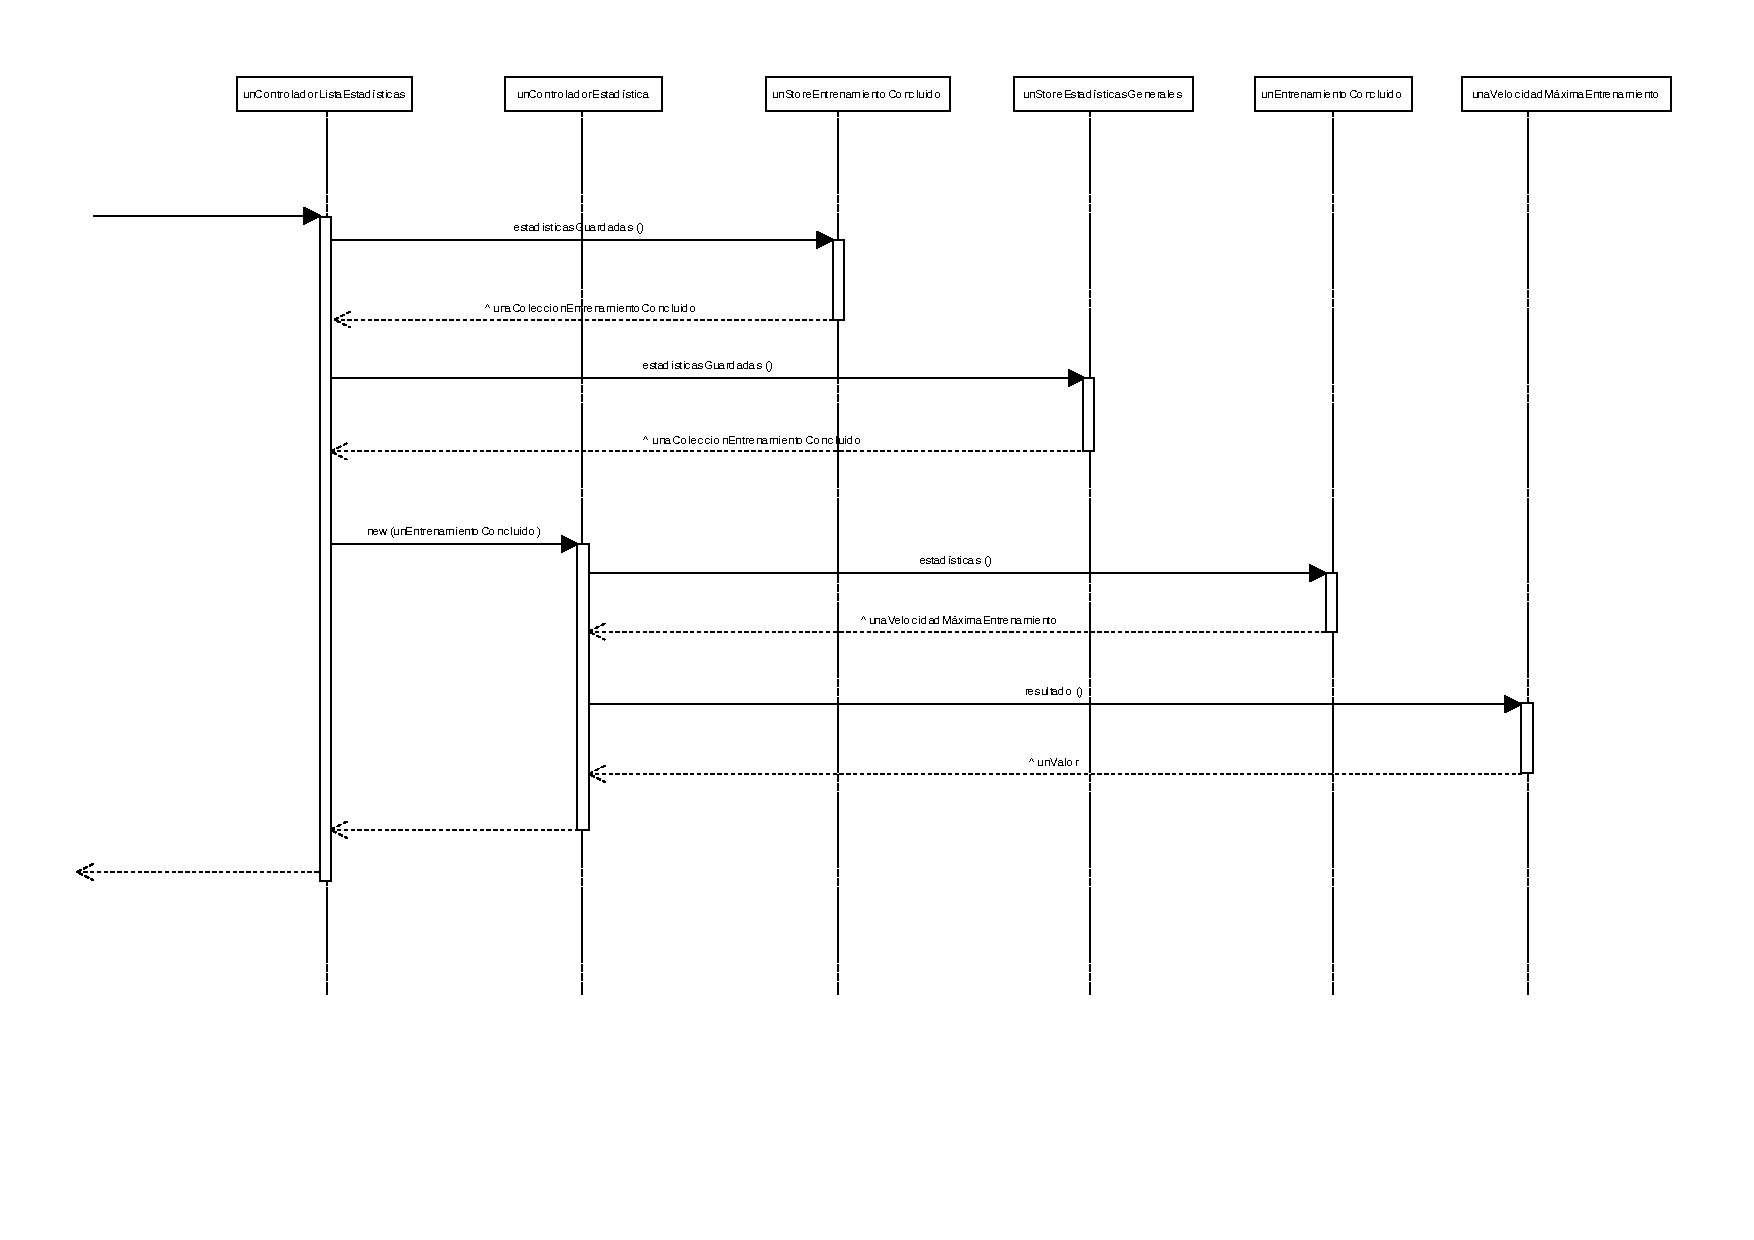
\includegraphics[scale=0.5]{images/ListadoEstadisticas.pdf}
\end{center}


Este diagrama explica el proceso que ocurre al mostrar las estadísticas particulares de los entrenamientos y las generales. En este caso, el usuario decide ver las estadísticas de un entrenamiento (como se ve en el diagrama de clases, la única disponible es la velocidad máxima del entrenamiento).


En primer lugar el \texttt{ControladorListaEstadísticas} le pide las \emph{estadísticasGuardadas ()} a los dos store: \texttt{storeEntrenamientoConcluido} y \texttt{storeEstadísticasGenerales}. Luego, el usuario selecciona {unEntrenamientoConcluido}, con lo cual debería cambiarse de vista a la de las estadísticas de ese entrenamiento. Es así que se crea un \texttt{ControladorEstadística} a partir del entrenamiento concluido que seleccionó el usuario. Este contralador envía el mensaje \emph{estadísticas ()}, que retorna una \texttt{VelocidadMáximaEntrenamiento}. A continuación, el contralador manda el mensaje \emph{resultado ()} a \texttt{VelocidadMáximaEntrenamiento} y recibe el resultado correspondiente. 

\subsubsection{Notificar que la velocidad del usuario es demasiado baja dentro de un seguimiento}
\begin{center}
	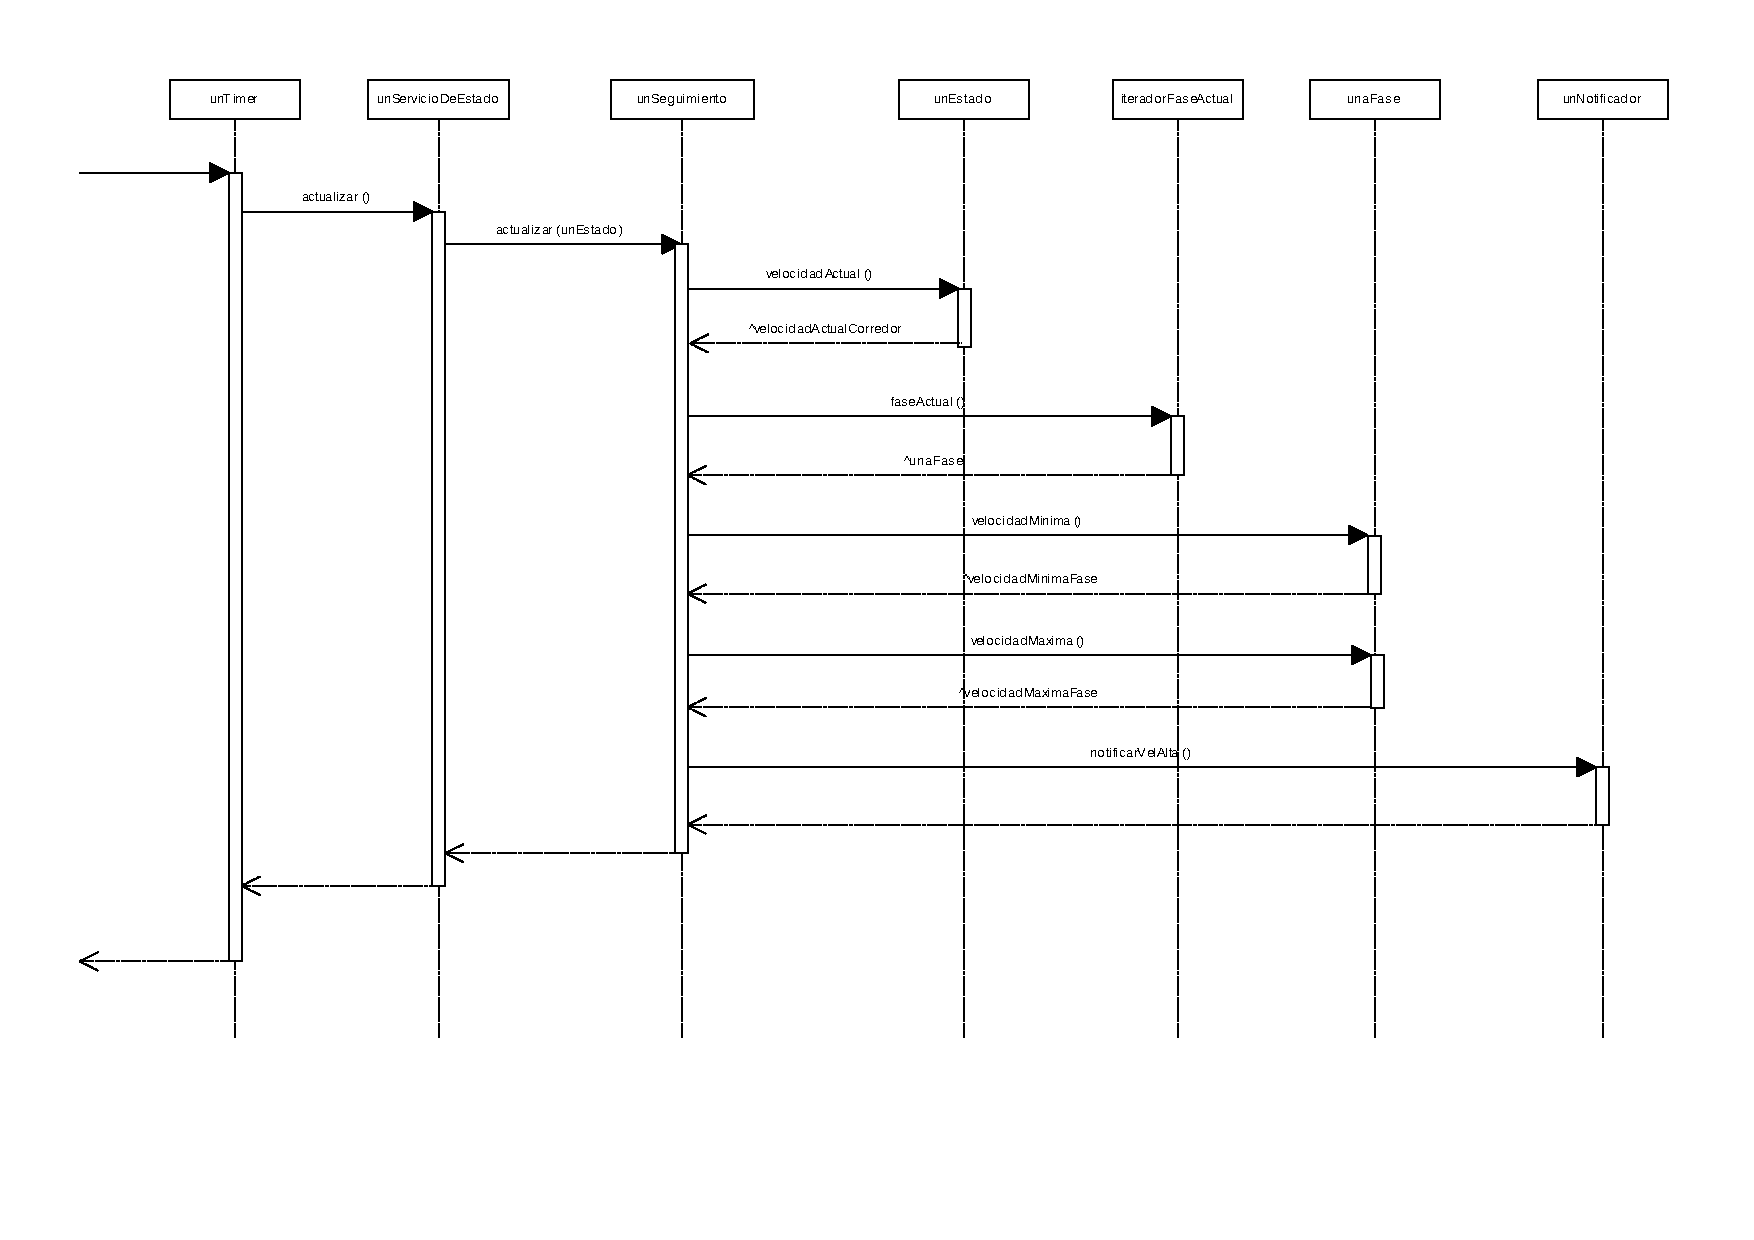
\includegraphics[scale=0.5]{images/Velocidad.pdf}
\end{center}

En este diagrama se observa el conjunto de mensajes que ocurren durante el un entrenamiento cuando el corredor se está desplazando más rápido de lo que su fase actual indica. Como se explicó en la sección \ref{unaSeccion}, cuando el \texttt{Timer} recibe el hipotético mensaje \emph{tic ()}, le avisa al \texttt{ServicioDeEstado} y éste le reporta a sus suscriptores (en particular al \texttt{Seguimiento}), el estado actual del corredor.

Cuando el \texttt{Seguimiento} recibe el mensaje \emph{actualizar (unEstado)}, extrae del parámetro la velocidad actual a la que se está desplazando el teléfono (enviándole al \texttt{Estado} el mensaje \emph{velocidadActual ()}) y le pide a su colaborador interno \texttt{IteradorDeFase} que le informe cuál es la fase actual, a la que le pregunta las velocidades mínima y máxima que corresponden a esa fase (mensajes \emph{velocidadMinima()} y \emph{velocidadMaxima ()} respectivamente).

Con esos tres datos, el \texttt{Seguimiento} verifica que la velocidad actual esté en rango y, suponiendo que no lo está (que está por encima de la máxima) le envía un mensaje a su colaborador interno \texttt{Notificador} diciéndole que notifique que la velocidad actual es muy alta (\emph{notificarVelAlta ()}). 

\subsubsection{Crear un plan básico}
\begin{center}
	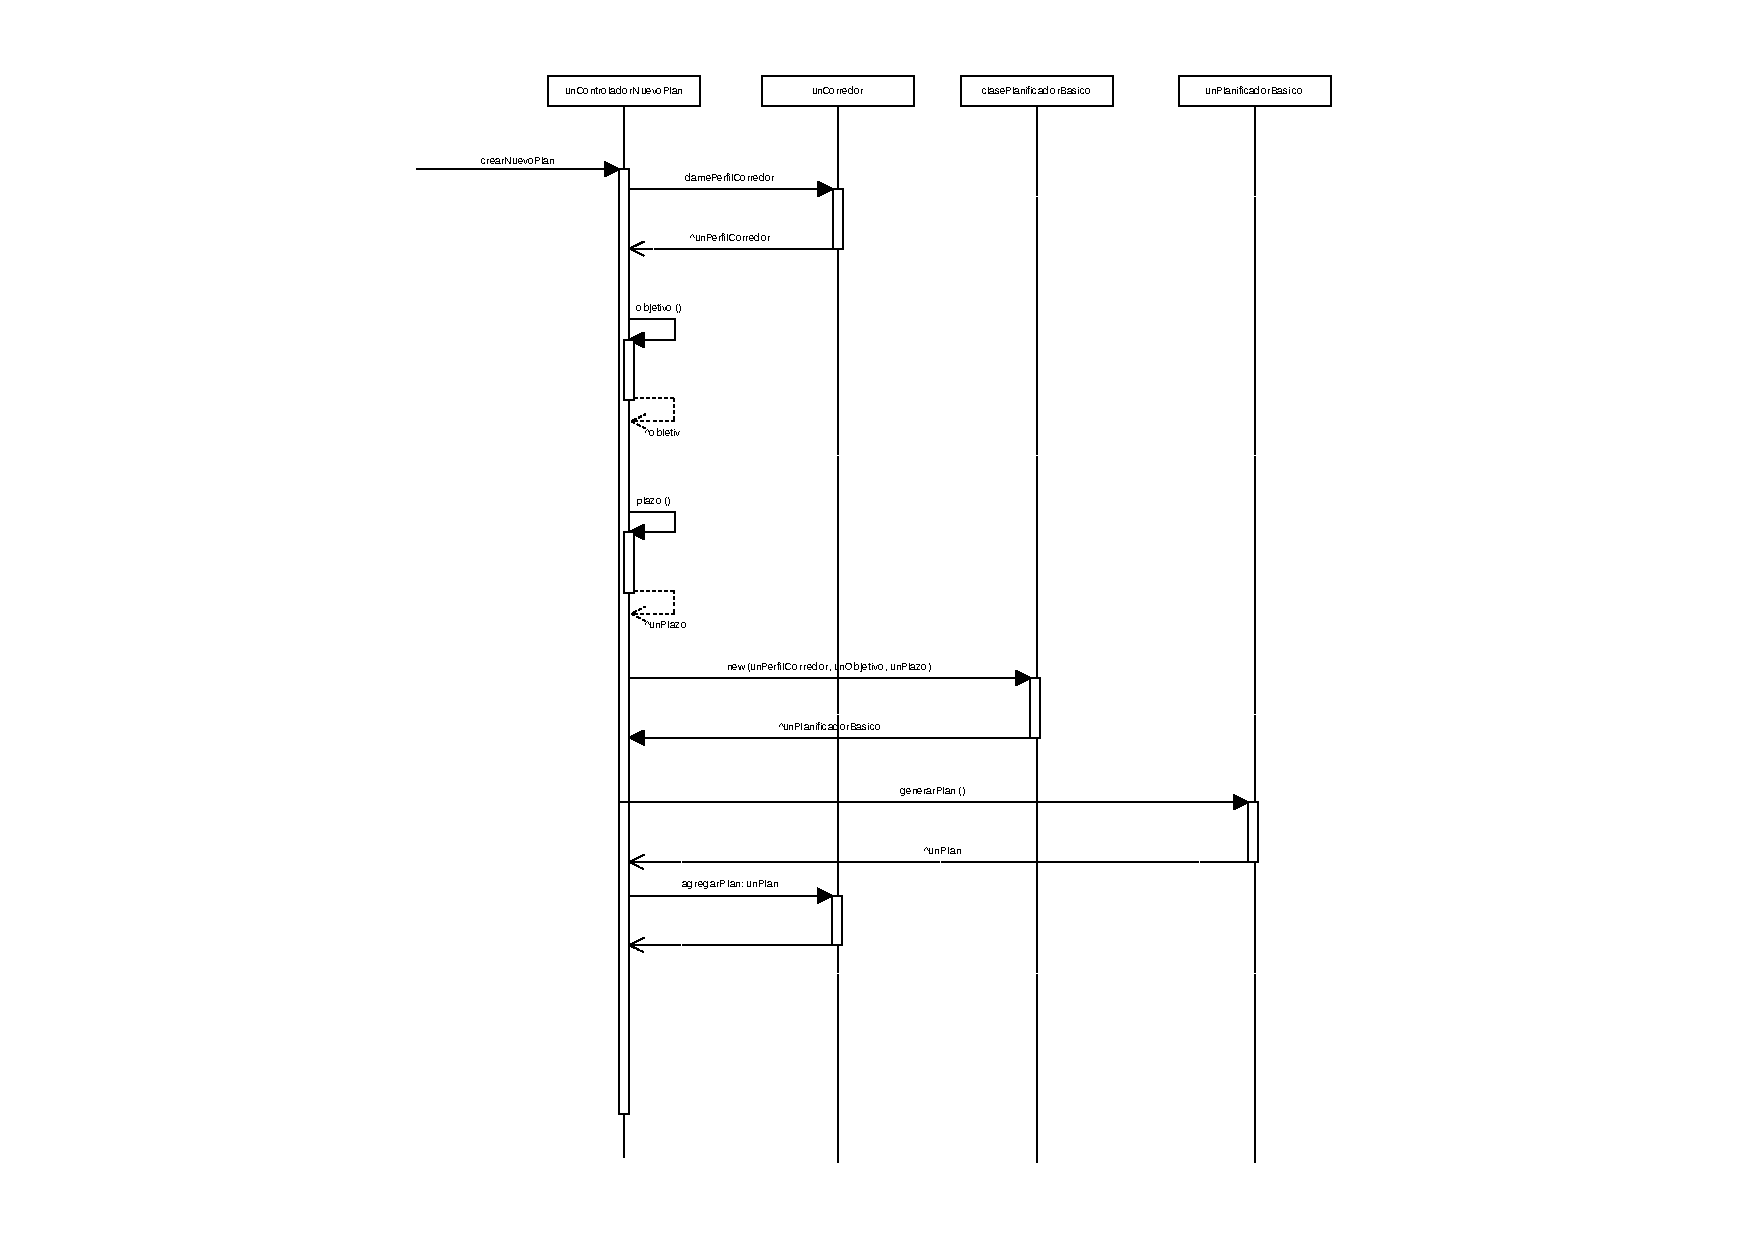
\includegraphics[scale=0.5]{images/PlanBasico.pdf}
\end{center}

Este diagrama representa el conjunto de mensajes que se intercambian a la hora de crear un plan nuevo. Si bien la creación en si misma está abstraida en un mensaje (\emph{generarPlan ()}) este diagrama muestra cómo el \texttt{ControladorNuevoPlan} obtiene los parámetros necesarios para crear el \texttt{Planificador} que, al recibir \emph{generarPlan ()} va a construir una instancia de \texttt{Plan}. 

Tanto el \texttt{Objetivo} como el \texttt{Plan} son colaboradores internos del \texttt{ControladorNuevoPlan}, mientras que el perfil de corredor lo obtiene enviándole el mensaje \emph{damePerfilCorredor ()} al objeto \texttt{unCorredor}.